% Chapter 2

\chapter{State of the Art} % Main chapter title
\label{chap:Chapter2} % For referencing the chapter elsewhere, use \ref{chap:Chapter2}

%----------------------------------------------------------------------------------------

This chapter reviews research on the automatic analysis of student responses, with emphasis on (i) Natural Language Processing (NLP) for educational assessment, (ii) error detection and correction in student writing, (iii) mathematical error analysis and misconception modeling, and (iv) synthetic data strategies for data-scarce educational settings. It places the thesis within established evaluation practices and modeling paradigms, points out gaps in current work, and states what the thesis contributes \parencite{Bryant2023GECsurvey,Woolf2010,RomeroVentura2024}.

\section{NLP for education and automated assessment}
\label{sec:sota_nlp_edu}

To place the thesis within established practice, this section looks at how Natural Language Processing (NLP) has been applied to educational assessment. The account is historical first. It then moves to the benchmarks and shared tasks used to compare systems, the architectures used for assessment and diagnosis, and the language coverage and deployment gaps that remain beyond English.

\subsection{Historical evolution of NLP in education}
\label{sec:sota_nlp_edu_history}

Automated assessment has passed through several distinct technical paradigms (Figure~\ref{fig:nlp_evolution}).

\begin{figure}[ht]
\centering
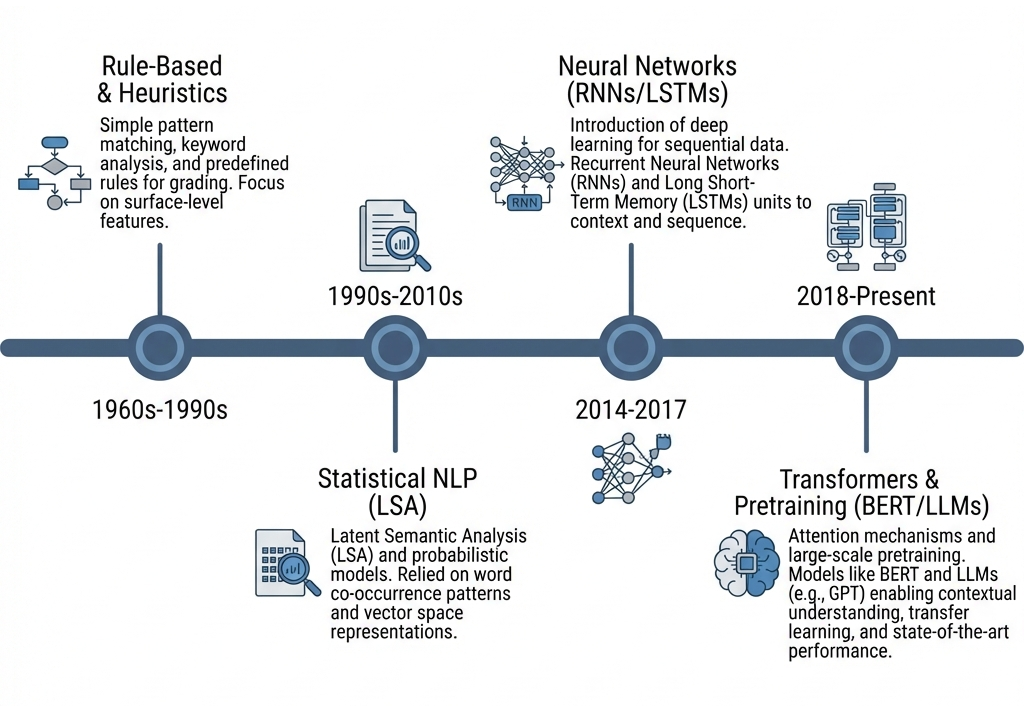
\includegraphics[width=1.0\textwidth]{figures/nlp_evolution_timeline.png}
\caption{Timeline showing the evolution of automated assessment from rule-based heuristics to modern Transformer-based architectures.}
\label{fig:nlp_evolution}
\end{figure}

Educational NLP initially focused on rule-based spell checking and grammar checking embedded in writing tools. These systems provided scalable surface-level feedback but offered limited diagnostic insight into why learners struggle. With the rise of Automated Essay Scoring (AES) and Automated Writing Evaluation (AWE), models increasingly learned to predict holistic or rubric-aligned scores from linguistic features extracted from corpora of human-scored responses. This motivated datasets for grading open-ended student writing such as the FCE corpus \parencite{YannakoudakisBriscoeMedlock2011,Bryant2023GECsurvey}.

Neural sequence models then enabled finer-grained signals, such as token-level error detection posed as a sequence labeling problem \parencite{ReiYannakoudakis2016}. In parallel, transformer architectures and large-scale pretraining shifted many educational NLP pipelines toward contextual representations that transfer across tasks. This shift improved scoring and feedback components \parencite{Vaswani2017,Devlin2019,Liu2019RoBERTa}. More recently, educational systems increasingly align with the ITS perspective in which assessment is coupled with difficulty identification and personalization: observed errors are mapped to hypotheses about missing skills and used to select adaptive interventions \parencite{Woolf2010,VanLehn2006}.

\subsection{Foundational benchmarks and shared tasks}
\label{sec:sota_nlp_edu_benchmarks}

Benchmark datasets and shared tasks provide reproducible protocols for comparing educational NLP systems under shared evaluation assumptions. In GEC, the CoNLL-2014 shared task standardized evaluation on the NUCLE learner corpus (57{,}151 training sentences; 1{,}312 test sentences) using edit-based scoring with the \(M^2\) scorer and the precision-weighted \(F_{0.5}\) metric \parencite{Ng2014,DahlmeierNg2012}. CoNLL-style data also carries an intrinsic educational constraint. Error sparsity (only a small fraction of tokens require edits) makes naive accuracy misleading and increases the risk of harmful overcorrection \parencite{Ng2014}.

BEA-2019 broadened evaluation by combining data sources such as Write\&Improve and LOCNESS (approximately 34{,}000 annotated examples) and by encouraging typed analyses via automatic error annotation frameworks like ERRANT \parencite{Bryant2019,BryantFeliceBriscoe2017}. Complementary resources such as JFLEG shift emphasis toward fluency-oriented rewriting with multiple human references, so that evaluation follows perceived writing quality more closely \parencite{Napoles2017}. Methodologically, these benchmarks define metrics and analysis practices that this thesis adapts for fine-grained analysis beyond end-to-end correction \parencite{Ng2014,Bryant2019}.

\subsection{Architectures and methods for assessment and diagnosis}
\label{sec:sota_nlp_edu_methods}

For formative applications, models must output interpretable signals at fine granularity (e.g., token- or span-level error tags) so that errors can be marked in the text, categorized, and aggregated into actionable summaries for teachers and learners \parencite{ReiYannakoudakis2016,BryantFeliceBriscoe2017}. Neural sequence labeling provides a well-established approach: bidirectional LSTMs capture contextual dependencies, CRF decoders enforce local label consistency, and character-aware encoders improve robustness to spelling variation \parencite{HochreiterSchmidhuber1997,HuangXuYu2015,MaHovy2016}.

Transformer pretraining further improves representations for scoring and labeling, while multilingual pretraining supports transfer to languages with limited labeled educational data \parencite{Devlin2019,Liu2019RoBERTa,Conneau2020}. Recent surveys synthesize neural and Transformer-based GEC systems and point to the growing use of synthetic data and data weighting to make use of heterogeneous corpora \parencite{Bryant2023GECsurvey,Lichtarge2020}.

\subsection{Beyond English: language coverage and deployment gaps}
\label{sec:sota_nlp_edu_beyond_english}

Despite substantial progress, the empirical ecosystem for error-centric educational NLP is still dominated by a small number of benchmark settings and genres, which shapes both modeling choices and evaluation practice \parencite{Ng2014,Bryant2019,BryantFeliceBriscoe2017}. Extending systems to new instructional contexts often requires rethinking annotation guidelines, label sets, and the mapping from model outputs to pedagogically meaningful categories. The interpretation of ``errors'' is inseparable from task design, curriculum expectations, and feedback goals \parencite{Bryant2023GECsurvey,Woolf2010}.

Recent work on Portuguese shows both progress and open questions. \textcite{Akef2026} combine LLM-based correction of European Portuguese learner writing with a rule-based module that characterizes 252 grammatical properties by the proficiency level at which they are taught, and use the resulting features for interpretable proficiency assessment. \textcite{Cabral2026} propose a synthetic dataset for spelling and grammar correction in Brazilian Portuguese and report that higher error-detection rates from offline LLMs do not necessarily reflect better performance and often signal overcorrection.

This motivates a thesis stance that prioritizes formative outputs that remain interpretable under distribution shift (token- and span-level predictions, typed error summaries, aggregation across tasks) and do not rely only on end-to-end corrected text \parencite{BryantFeliceBriscoe2017,Ng2014}. In practice, this means adopting benchmark-informed metrics and analysis tools while explicitly validating them under the intended educational use case, consistent with the ITS view that assessment must connect to actionable pedagogical hypotheses \parencite{Woolf2010,VanLehn2006}.


\section{Error detection and correction in writing}
\label{sec:sota_gec}

Error detection and correction in written text is the task closest to the linguistic module of the thesis, so it gets a section of its own. The first subsection covers the approaches to Grammatical Error Correction (GEC) and how they are evaluated. Neural architectures for error detection come next, followed by the problems of data scarcity, domain shift and data weighting, and finally learner corpora and error annotation beyond benchmark settings.

\subsection{Grammatical Error Correction (GEC): landscape and evaluation}
\label{sec:sota_gec_landscape}

Different technical paradigms for GEC offer distinct trade-offs between precision, fluency, and interpretability (Table~\ref{tab:gec_approaches}).

\begin{table}[ht]
\centering
\caption{Comparison of the main approaches to Grammatical Error Correction (GEC).}
\label{tab:gec_approaches}
\begin{tabular}{p{0.2\textwidth}p{0.3\textwidth}p{0.4\textwidth}}
\toprule
\textbf{Approach} & \textbf{Mechanism} & \textbf{Pros (+) and Cons (-)} \\
\midrule
Rule-based & Hand-crafted linguistic rules & (+) High precision, explainable \\
& & (-) Low recall, brittle to unseen errors \\
\midrule
SMT (Statistical) & Phrase-based translation & (+) Learned from data \\
& & (-) Requires large parallel corpora, limited context \\
\midrule
NMT (Neural) & Seq2Seq deep learning & (+) Better fluency, handles complex errors \\
& & (-) ``Black box'', needs massive training data \\
\midrule
LLM-based & Prompting (zero- or few-shot) & (+) No task-specific training needed, high fluency \\
& & (-) Hallucinations, hard to control specific error types \\
\bottomrule
\end{tabular}
\end{table}

Grammatical Error Correction (GEC) is commonly formulated as transforming an erroneous input sentence into a corrected output sentence, whereas grammatical error detection focuses on identifying error locations (and, ideally, types) without necessarily generating a full correction \parencite{Ng2014,ReiYannakoudakis2016}. In educational settings, this distinction is substantive: correction optimizes end-to-end output quality, while detection supports interpretable signals for marking errors and for aggregation \parencite{BryantFeliceBriscoe2017,Bryant2023GECsurvey}.

Benchmark evaluation reflects the asymmetric cost of mistakes in learner-facing systems. CoNLL-style evaluation relies on edit matching and reports the precision-weighted \(F_{0.5}\) score, which prioritizes avoiding harmful false corrections \parencite{DahlmeierNg2012,Ng2014}. Formally, \(F_{0.5} = (1+0.5^2)\frac{PR}{0.5^2P+R}\), where \(P\) and \(R\) denote precision and recall \parencite{DahlmeierNg2012}. Modern practice complements aggregate scores with typed analyses (e.g., ERRANT categories) to understand which error types systems handle reliably \parencite{Bryant2019,BryantFeliceBriscoe2017}.

\subsection{Neural architectures for error detection}
\label{sec:sota_gec_arch}

Token-level error detection is naturally modeled as sequence labeling, where each token receives a label indicating correctness or a finer-grained error category. Architectures typically combine contextual encoding with structured decoding to produce coherent label sequences \parencite{HochreiterSchmidhuber1997,HuangXuYu2015}. A widely adopted blueprint is the BiLSTM-CNN-CRF architecture, which integrates character-level features with contextual BiLSTM representations and CRF decoding \parencite{MaHovy2016}. Empirically, \textcite{MaHovy2016} reported strong results in canonical sequence-labeling tasks, and the architecture is a strong baseline for token-level prediction.

For learner writing, \textcite{ReiYannakoudakis2016} demonstrated that neural sequence labeling achieves competitive error detection performance while producing token-level decisions suitable for pedagogical aggregation \parencite{ReiYannakoudakis2016,BryantFeliceBriscoe2017}. Character-aware modeling is useful under authentic spelling variation, since character-level representations allow a sequence labeler to generalize to unseen or misspelled word forms \parencite{MaHovy2016}.

In parallel, transformer-based modeling supports both detection and correction. Pretrained encoders accept fine-tuning for token-level tagging, while text-to-text transformers offer a unified framework in which correction is posed as conditional generation \parencite{Devlin2019,Liu2019RoBERTa,Raffel2020}. Large Language Models (LLMs) have also demonstrated state-of-the-art capabilities in GEC, acting as strong correctors or error generators, though challenges remain regarding controllability and hallucination \parencite{CoyneSakaguchi2023,Bryant2023GECsurvey}. Recent work shows that GPT-style LLMs can outperform traditional GEC systems while also exposing weaknesses in reference-based evaluation \parencite{CoyneSakaguchi2023}. Other studies deploy GEC directly in language learning exercises and show that error-correction systems can support sentence-level assessment and formative feedback \parencite{Katinskaia2023}.

\subsection{Data scarcity, domain shift, and data weighting}
\label{sec:sota_gec_data}

High-quality learner corpora with fine-grained annotation are costly to produce, and performance depends strongly on alignment between training data and the target educational domain \parencite{Ng2014,Bryant2019,Bryant2023GECsurvey}. Data-weighted training offers one principled mechanism for using large heterogeneous corpora while favoring examples that better match the target distribution \parencite{Lichtarge2020}.

Recent work shows that weighting heterogeneous data and using synthetic error corpora can substantially improve GEC performance \parencite{Lichtarge2020,Bryant2023GECsurvey}. Concretely, \textcite{Lichtarge2020} proposes a data-weighting approach based on delta log perplexity, which assigns higher weights to examples similar to a high-quality target dataset. Large-scale synthetic parallel data is another way to expand training signal when authentic learner data is limited, although the pedagogical validity of synthetic error distributions requires verification for the target population \parencite{Bryant2023GECsurvey}.

\subsection{Learner corpora and error annotation beyond benchmark settings}
\label{sec:sota_gec_corpora}

High-quality learner corpora and error annotations are a prerequisite for reliable evaluation and diagnostic feedback, yet they are expensive to develop and difficult to standardize across educational settings \parencite{Bryant2023GECsurvey,Ng2014}. Beyond widely used English benchmarks, researchers must typically define annotation guidelines that are aligned with local pedagogical goals, establish error-type inventories that support interpretability, and design validation procedures that make performance claims meaningful \parencite{Bryant2023GECsurvey,Woolf2010}.

At the evaluation level, typed analyses are valuable because they reveal whether improvements in aggregate scores are driven by common ``easy'' categories or whether models are reliable on pedagogically salient phenomena \parencite{BryantFeliceBriscoe2017,Bryant2019}. In practice, this motivates reporting both precision-weighted metrics for correction and error-type breakdowns for difficulty identification \parencite{DahlmeierNg2012,Ng2014}.

\section{Mathematical error analysis and feedback systems}
\label{sec:sota_math}

Student errors in mathematics often follow systematic patterns, so this section turns to that domain. Its four parts cover taxonomies of mathematical errors, the shift from final-answer grading to the analysis of process data, data-driven discovery of misconceptions and longitudinal patterns, and the architecture and feedback design of Intelligent Tutoring Systems (ITS).

\subsection{Taxonomies of mathematical errors}
\label{sec:sota_math_tax}

Unlike many language tasks where correctness is graded at the sentence level, mathematics assessment often requires analyzing intermediate steps and reasoning traces. Educational psychology and cognitive modeling distinguish several kinds of errors. Early computational models of ``bugs'' in procedural skills treat recurring mistakes as manifestations of incorrect rules that students apply systematically \parencite{BrownBurton1978,VanLehn1990}.

In this tradition, a useful distinction lies between conceptual errors (misunderstanding underlying principles), procedural errors (mis-executing an algorithm despite correct conceptual intent), and computational slips (isolated arithmetic mistakes), a distinction that echoes the divide between conceptual and procedural knowledge in mathematics education \parencite{VanLehn1990,RittleJohnson2015}. A study of elementary teachers analyzing subtraction errors found that they could describe specific error patterns but did not base their instructional focus on them \parencite{Riccomini2005}.

\subsection{From final-answer grading to process data}
\label{sec:sota_math_process}

Difficulty identification in mathematics benefits from process data: intermediate steps, action sequences, and the structure of solution traces. ITS research holds that step-level analysis enables immediate feedback and more accurate inference about student knowledge states than final-answer correctness alone \parencite{Woolf2010,VanLehn2006}. In classic tutoring architectures, such identification links observed actions to hypothesized misconceptions or missing skills \parencite{BrownBurton1978,VanLehn1990}.

Formal student modeling provides additional mechanisms to represent learning over time. Knowledge tracing models procedural skill acquisition as a latent state that evolves with practice, so that systems can estimate mastery and select appropriate problems \parencite{CorbettAnderson1995,Piech2015}. These approaches provide a methodological basis for longitudinal analysis of learning difficulties, but they depend on reliable extraction of error signals and step representations from student work \parencite{Woolf2010,Piech2015}.

\subsection{Data-driven misconception discovery and longitudinal patterns}
\label{sec:sota_math_misconceptions}

When expert-defined bug libraries are unavailable or incomplete, educational data mining offers alternative mechanisms for discovering patterns in student errors. Reviews of educational data mining stress clustering, pattern mining, and predictive modeling as ways to identify common failure modes and to support teacher-facing analytics at scale \parencite{BakerYacef2009,RomeroVentura2010EDM}. More recent EDM reviews note that these techniques remain relevant for identifying persistent student difficulties \parencite{RomeroVentura2024}. Recent bibliometric analyses confirm that prediction of student performance, clustering, and learning analytics remain core EDM topics with growing attention to personalized learning systems \parencite{Rao2024}.

Longitudinal analysis is relevant for the present thesis because learning difficulties are often defined by persistence and recurrence. Reliable profiling requires aggregating evidence across tasks and time \parencite{BakerYacef2009,RomeroVentura2024}. This points to a pipeline in which error signals are extracted at fine granularity and aggregated into stable patterns for validation against pedagogical expectations \parencite{Woolf2010}.

\subsection{ITS architectures and feedback design}
\label{sec:sota_math_its}

Across domains, ITS architectures share a common pipeline: student modeling, difficulty detection, decision-making, and feedback delivery \parencite{Woolf2010}. Reviews of tutoring system behavior report that the effectiveness of feedback depends on matching interventions to the learner's underlying difficulty \parencite{VanLehn2006}. In school settings, the design challenge is to produce feedback that is both timely and instructionally aligned \parencite{KoedingerAnderson1997,Woolf2010}.

Recent systems such as LPITutor demonstrate how LLM-based personalized tutoring can use retrieval-augmented generation (RAG) and prompt engineering to support personalized feedback and adaptive instruction \parencite{LPITutor2025}. These emerging approaches illustrate the potential for integrating error detection with conversational tutoring interfaces. In mathematics specifically, MathDial pairs human teachers with an LLM instructed to simulate typical learner mistakes. The result is roughly 3{,}000 tutoring dialogues on mathematical reasoning problems, and models fine-tuned on them make more effective tutors \parencite{Macina2023MathDial}. This thesis adopts similar principles and treats error detection as an enabling component for pedagogical feedback.

\section{Synthetic data and data scarcity in educational AI}
\label{sec:sota_synth}

Educational data is scarce, sensitive and costly to annotate, which is what motivates the use of synthetic data. The section starts with the scarcity problem in educational NLP and then covers two families of generation methods, rule-based and LLM-based. It ends with the criteria used to judge whether synthetic data actually helps.

\subsection{The data scarcity problem in educational NLP}
\label{sec:sota_synth_scarcity}

Annotated educational corpora are expensive to produce and often limited in scale compared to general-domain NLP resources, creating a large data gap (Figure~\ref{fig:data_scarcity}).

\begin{figure}[ht]
\centering
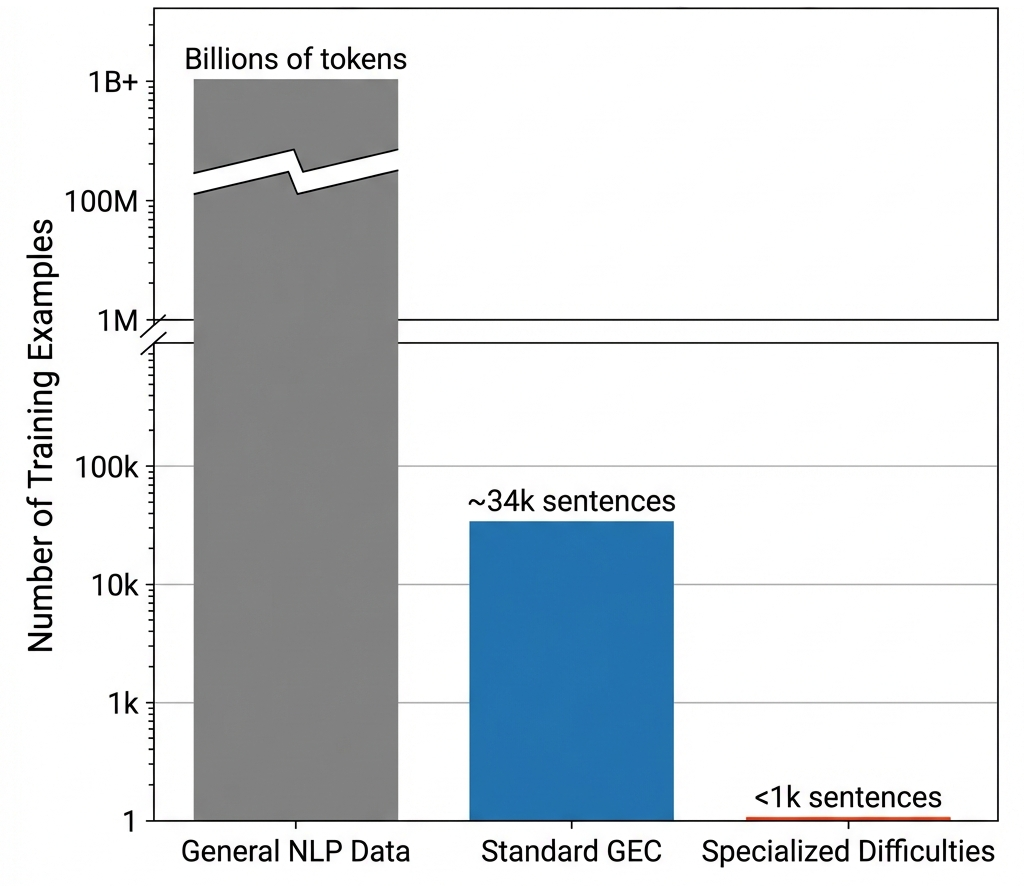
\includegraphics[width=0.7\textwidth]{figures/data_scarcity.png}
\caption{Comparison of training data availability showing the orders-of-magnitude gap between general NLP, standard GEC, and specialized difficulty domains.}
\label{fig:data_scarcity}
\end{figure}

The NUCLE corpus, used in CoNLL-2014, contains approximately 57,000 sentences; the FCE corpus roughly 30,000 sentences; and the combined BEA-2019 training pool approximately 34,000 examples \parencite{Ng2014,Bryant2019,YannakoudakisBriscoeMedlock2011}. These datasets, while valuable, are small relative to general pretraining corpora and concentrated on specific learner populations. For K--12 education, difficulty-specific error patterns, and languages other than English, labeled data is even scarcer \parencite{Joshi2020,Bryant2023GECsurvey}.

\subsection{Rule-based synthetic error generation}
\label{sec:sota_synth_rule}

Rule-based corruption provides a controlled mechanism for generating synthetic training data by systematically transforming correct text into errorful versions. In GEC research, noise injection methods include random character operations (insertions, deletions, substitutions, transpositions), word-level swaps, and rule-based grammatical corruptions \parencite{Lichtarge2020}. These approaches generate large volumes of parallel data but risk producing error distributions that do not match authentic learner behavior.

For difficulty-linked patterns, rule-based generation is more theory-informed. Phonological substitution rules implement systematic voiced/voiceless consonant swaps (e.g., /p/$\leftrightarrow$/b/, /t/$\leftrightarrow$/d/) based on documented confusion patterns in dyslexia research \parencite{ShaywitzShaywitz2005}. Orthographic corruption rules target specific phenomena such as consonant doubling errors, silent letter omissions, and homophone confusions.

\subsection{LLM-based synthetic data generation}
\label{sec:sota_synth_llm}

Large Language Models offer an alternative mechanism for generating synthetic educational data. LLMs produce learner-like text with specific error patterns when prompted, potentially capturing stylistic and contextual properties that rule-based methods miss \parencite{Brown2020,Ouyang2022}. Several approaches exist: (i) direct prompting, where LLMs generate responses ``as if written by a student with specific difficulties''; (ii) controlled generation with conditioning signals to specify target error types; and (iii) hybrid approaches where LLMs generate base responses that are then corrupted using rule-based methods to keep the labels accurate.

Recent studies confirm that LLMs can act as strong error generators and correctors \parencite{CoyneSakaguchi2023,Bryant2023GECsurvey}. Fine-tuning an open LLM (Llama~2) to generate errors has been shown to yield synthetic errors similar to human errors and, when these are used to train correction models, to improve on previous state-of-the-art results for German, Ukrainian, and Estonian \parencite{Luhtaru2024}. LLM-generated synthetic data also carries risks. Generated errors may not match authentic learner distributions, and models may hallucinate implausible patterns. Quality control (human review of samples, comparison against authentic error distributions, and validation of label accuracy) is needed before LLM-generated data is used for training educational systems \parencite{Bryant2023GECsurvey}. These cautions echo wider discussions of the opportunities and challenges of LLMs in education \parencite{Kasneci2023}.

\subsection{Evaluating synthetic data effectiveness}
\label{sec:sota_synth_eval}

The effectiveness of synthetic data depends on alignment between the synthetic distribution and the target deployment population. \textcite{Lichtarge2020} demonstrated that data weighting improves GEC performance by giving more weight to training examples similar to the target distribution. In educational settings, validation implies distribution analysis (comparing error-type frequencies in synthetic and authentic data), transfer evaluation, and generalization checks. The thesis follows these evaluation principles by explicitly comparing models trained with and without synthetic augmentation \parencite{Lichtarge2020,Bryant2023GECsurvey}.

\section{Learning difficulties, profiles, and ethical considerations}
\label{sec:sota_ethics}

The last building block of the thesis is how learning difficulties can be approached computationally without making clinical claims. The subsections below start with computational approaches to learning difficulty detection, move to student profiling and cluster-based analytics, and end with the ethical constraints and non-clinical framing that guide the design of the system.

\subsection{Computational approaches to learning difficulty detection}
\label{sec:sota_ethics_detect}

A growing body of research explores computational methods for detecting indicators of learning difficulties from digital traces. In reading and writing, research has characterized the distribution of errors in text written by learners with dyslexia and contrasted it with that of typically developing peers \parencite{ShaywitzShaywitz2005,RelloBaezaYates2014}. While this research shows that certain error patterns (phonological substitutions, orthographic inconsistencies, and segmentation difficulties) occur more frequently in individuals with dyslexia, it also reports substantial individual variation and overlap between populations. A recent systematic review of machine-learning-based dyslexia screening draws mainly on signals such as electroencephalographic recordings, eye-tracking, and handwriting analysis \parencite{JanKhan2023}, which differ from the typed, text-only setting adopted in this thesis.

In mathematics, research on dyscalculia and math learning difficulties identified characteristic error patterns, including difficulties with number magnitude comparison, procedural bugs in arithmetic, and fraction misconceptions \parencite{VanLehn1990,BrownBurton1978}. These patterns work as proxies or risk indicators, but they do not constitute diagnostic criteria in clinical or educational-psychological terms.

\subsection{Student profiling and cluster-based analytics}
\label{sec:sota_ethics_profiles}

Educational data mining offers methods for aggregating error signals into student profiles. Clustering algorithms (e.g., k-means, hierarchical clustering) group students by similarity in error distributions and can reveal subgroups with distinct difficulty patterns \parencite{BakerYacef2009,RomeroVentura2010EDM}. Knowledge tracing and its neural variants model skill acquisition over time \parencite{CorbettAnderson1995,Piech2015}.

For teacher-facing analytics, profiles have to be interpretable. Clusters should correspond to actionable pedagogical categories, not opaque statistical groupings, and validation against educator intuition and external assessments is necessary \parencite{RomeroVentura2024}. Profile labels must avoid stigmatizing language and should frame patterns as areas for instructional attention and not present them as fixed student attributes.

\subsection{Ethical constraints and non-clinical framing}
\label{sec:sota_ethics_ethical}

The application of AI to detecting learning difficulties raises serious ethical concerns that this thesis addresses directly. First, the framing must be non-clinical. Automated systems cannot and should not provide clinical diagnoses of dyslexia, dyscalculia, or other learning disabilities. Diagnosis requires a full assessment by qualified professionals \parencite{ShaywitzShaywitz2005}. This thesis frames system outputs as \emph{pedagogical indicators} that may warrant further attention, not diagnostic labels.

Second, system outputs are designed for teacher review and interpretation, not for automated decision-making about students \parencite{Woolf2010}.

Third, data protection and privacy need attention. Educational data is sensitive, and more so when it is linked to potential learning difficulties. Processing requires compliance with relevant regulations, above all the General Data Protection Regulation (GDPR) \parencite{EU2016GDPR}, including data minimization, purpose limitation, and appropriate security. In addition, AI systems intended to evaluate learning outcomes, including when these are used to steer the learning process, are classified as high-risk under Annex~III (point~3(b)) of the European Artificial Intelligence Act \parencite{EU2024AIAct}. Although this thesis targets formative, teacher-reviewed indicators rather than grading or admission decisions, this classification reinforces the need for human oversight, transparency, and careful data governance.

Finally, labeling students with difficulty indicators risks stigmatization if misused. System design should use growth-oriented framing and avoid deficit framing. A recent systematic review of fairness, accountability, transparency, and ethics in AI for higher education finds that fairness receives substantially more attention than accountability or transparency \parencite{MemarianDoleck2023}. This supports the emphasis placed here on transparent, teacher-reviewable outputs.

\section{Identified gaps and thesis contribution}
\label{sec:sota_gaps}

The review above points to three gaps in the literature: underrepresented languages and local educational contexts, the limited use of synthetic data for difficulty-linked error patterns, and the scarcity of longitudinal analysis beyond single responses. Each gets its own subsection, together with a statement of how the thesis addresses it. The section closes by positioning the integrated contribution of the thesis with respect to these gaps.

\subsection{Gap 1: Underrepresented languages and local educational contexts}
\label{sec:sota_gap_pt}

The most mature evaluation ecosystems for error-centric educational NLP are centered on a small set of widely used learner corpora and shared tasks \parencite{Ng2014,Bryant2019,BryantFeliceBriscoe2017}. Extending these methods requires aligning label inventories and evaluation protocols with the intended pedagogical use, especially when outputs must be interpretable for teacher review \parencite{Bryant2023GECsurvey,Woolf2010}. The scarcity of resources in specific languages further complicates this, as noted by \textcite{Joshi2020}. Recent studies on Portuguese pursue proficiency assessment \parencite{Akef2026} and general spelling and grammar correction \parencite{Cabral2026}; as far as the reviewed literature shows, they do not target difficulty-linked error patterns in school-age writing.

The thesis responds with formative outputs (error locations and types) that aggregate across tasks and time, and with evaluation grounded in benchmark-informed metrics that are explicitly validated for the local educational context.

\subsection{Gap 2: Limited use of synthetic data for difficulty-linked error patterns}
\label{sec:sota_gap_synth}

While synthetic error generation has been explored in general GEC research, including recent LLM-based approaches \parencite{Luhtaru2024}, its application to difficulty-linked error patterns (those specifically associated with learning difficulties such as dyslexia or dyscalculia) remains underexplored \parencite{Lichtarge2020,Bryant2023GECsurvey}. Existing approaches typically generate generic grammatical errors rather than the systematic phonological, orthographic, and segmentation patterns that research connects to persistent learning difficulties \parencite{ShaywitzShaywitz2005}.

To address this gap, the thesis designs theory-informed, rule-based synthetic data generators that produce error patterns aligned with established taxonomies of learning difficulties \parencite{Bryant2023GECsurvey}; LLM-based generation was considered and, for the reasons given in Section~\ref{sec:method_data_llm}, not adopted.

\subsection{Gap 3: Longitudinal difficulty patterns beyond single responses}
\label{sec:sota_gap_long}

Most benchmark evaluations in error detection and correction focus on sentence-level or essay-level outcomes, while educational practice often requires longitudinal evidence to distinguish episodic mistakes from persistent learning difficulties \parencite{RomeroVentura2024}.

Here the thesis models error recurrence explicitly. Extracted error signals are aggregated over time and analyzed to identify stable profiles of difficulty, informed by educational data mining practices and longitudinal learning perspectives \parencite{BakerYacef2009,RomeroVentura2024}.

\subsection{Integrated thesis contribution and positioning}
\label{sec:sota_contrib}

By integrating error-centric NLP, symbolic mathematical analysis, theory-informed synthetic data, and longitudinal profiling, this thesis positions itself at the intersection of automated assessment and intelligent tutoring. Concretely, it builds on benchmark-driven evaluation practice for error-centric NLP, uses established sequence-labeling architectures for interpretable detection, and grounds feedback design in ITS principles that give priority to difficulty identification and actionable intervention \parencite{DahlmeierNg2012,Ng2014,BryantFeliceBriscoe2017,ReiYannakoudakis2016,MaHovy2016,Woolf2010}.

The intended outcome is a text-based system that (i) detects and classifies error patterns linked to learning difficulties in typed student responses, (ii) uses synthetic data to address data scarcity, and (iii) surfaces persistent difficulty patterns as interpretable, non-clinical profiles to support pedagogical decision-making \parencite{Bryant2023GECsurvey,RomeroVentura2024}.
